%%%%%%%%%%%%%%%%%%%%%%%%%%%%%%%%%%%%%%%%%
% eBook
% LaTeX Template
% Version 1.0 (29/12/14)
%
% This template has been downloaded from:
% http://www.LaTeXTemplates.com
%
% Original author:
% Luis Cobo (luiscobogutierrez@gmail.com) with extensive modifications by:
% Vel (vel@latextemplates.com)
%
% License:
% CC BY-NC-SA 3.0 (http://creativecommons.org/licenses/by-nc-sa/3.0/)
%
%%%%%%%%%%%%%%%%%%%%%%%%%%%%%%%%%%%%%%%%%

%----------------------------------------------------------------------------------------
%	DOCUMENT CONFIGURATIONS AND INFORMATION
%----------------------------------------------------------------------------------------

\documentclass[oneside,11pt]{memoir} % Font size

%%%%%%%%%%%%%%%%%%%%%%%%%%%%%%%%%%%%%%%%%
% eBook
% Structural Definitions File
% Version 1.0 (29/12/14)
%
% Created by:
% Vel (vel@latextemplates.com)
%
% This file has been downloaded from:
% http://www.LaTeXTemplates.com
%
% License:
% CC BY-NC-SA 3.0 (http://creativecommons.org/licenses/by-nc-sa/3.0/)
%
%%%%%%%%%%%%%%%%%%%%%%%%%%%%%%%%%%%%%%%%%

%----------------------------------------------------------------------------------------
%	REQUIRED PACKAGES
%----------------------------------------------------------------------------------------

\usepackage[utf8]{inputenc} % Required for inputting international characters
\usepackage[T1]{fontenc} % Output font encoding for international characters

\usepackage[osf]{libertine} % Use the Libertine font
\usepackage{microtype} % Improves character and word spacing

\usepackage{tikz} % Required for drawing custom shapes
\definecolor[named]{color01}{rgb}{.2,.4,.6} % Color used in the title page
\usepackage{wallpaper} % Required for setting background images (title page)

\usepackage[unicode=true,bookmarks=true,bookmarksnumbered=false,bookmarksopen=false,breaklinks=false,pdfborder={0 0 1},backref=section,colorlinks=false]{hyperref} % PDF meta-information specification
\usepackage{inputenc} % Accept different input encodings

%----------------------------------------------------------------------------------------
%	PAPER, MARGIN AND HEADER/FOOTER SIZES
%----------------------------------------------------------------------------------------

\setstocksize{12.5cm}{9.4cm} % Paper size
\settrimmedsize{\stockheight}{\stockwidth}{*} % No trims
\setlrmarginsandblock{18pt}{18pt}{*} % Left/right margins
\setulmarginsandblock{30pt}{36pt}{*} % Top/bottom margins
\setheadfoot{14pt}{12pt} % Header/footer height
\setheaderspaces{*}{8pt}{*} % Extra header space

%----------------------------------------------------------------------------------------
%	FOOTNOTE CUSTOMIZATION
%----------------------------------------------------------------------------------------

\renewcommand{\foottextfont}{\itshape\footnotesize} % Font settings for footnotes
\setlength{\footmarkwidth}{-.1em} % Space between the footnote number and the text
\setlength{\footmarksep}{.1em} % Space between multiple footnotes on the same page
\renewcommand*{\footnoterule}{} % Remove the rule above the first footnote
\setlength{\skip\footins}{1\onelineskip} % Space between the body text and the footnote

%----------------------------------------------------------------------------------------
%	HEADER AND FOOTER FORMATS
%----------------------------------------------------------------------------------------

\makepagestyle{mio} % Define a new custom page style
\setlength{\headwidth}{\textwidth} % Header the same width as the text
\makeheadrule{mio}{\textwidth}{0.1mm} % Header rule height
\makeoddhead{mio}{\scriptsize{\theauthor\hskip.2cm\vrule\hskip.2cm\itshape{\thetitle}}}{}{} % Header specification
\makeoddfoot{mio}{}{\scriptsize {\thepage \quad \vrule \quad \thelastpage}}{} % Footer specification
\makeoddfoot{plain}{}{\footnotesize {\thepage \quad \vrule \quad \thelastpage}}{} % Pages of chapters
\pagestyle{mio} % Set the page style to the custom style defined above

%----------------------------------------------------------------------------------------
%	PART FORMAT
%----------------------------------------------------------------------------------------

\renewcommand{\partnamefont}{\centering\sffamily\itshape\Huge} % Part name font specification
\renewcommand{\partnumfont}{\sffamily\Huge} % Part number font specification
\renewcommand{\parttitlefont}{\centering\sffamily\scshape} % Part title font specification
\renewcommand{\beforepartskip}{\null\vskip.618\textheight} % Whitespace above the part heading

%----------------------------------------------------------------------------------------
%	CHAPTER FORMAT
%----------------------------------------------------------------------------------------

\makechapterstyle{Tufte}{ % Define a new chapter style
\renewcommand{\chapterheadstart}{\null \vskip3.5\onelineskip} % Whitespace before the chapter starts
\renewcommand{\printchaptername}{\large\itshape\chaptername} % "Chapter" text font specification
\renewcommand{\printchapternum}{\LARGE\thechapter \\} % Chapter number font specification
\renewcommand{\afterchapternum}{} % Space between the chapter number and text
\renewcommand{\printchaptertitle}[1]{ % Chapter title font specification
\raggedright
\itshape\Huge{##1}}
\renewcommand{\afterchaptertitle}{
\vskip3.5\onelineskip
}}
\chapterstyle{Tufte} % Set the chapter style to the custom style defined above

%----------------------------------------------------------------------------------------
%	SECTION FORMAT
%----------------------------------------------------------------------------------------

\setsecheadstyle{\sethangfrom{\noindent ##1}\raggedright\sffamily\itshape\Large} % Section title font specification
\setbeforesecskip{-.6\onelineskip} % Whitespace before the section
\setaftersecskip{.3\onelineskip} % Whitespace after the section

%----------------------------------------------------------------------------------------
%	SUBSECTION FORMAT
%----------------------------------------------------------------------------------------

\setsubsecheadstyle{\sethangfrom{\noindent  ##1}\raggedright\sffamily\large\itshape} % Subsection title font specification
\setbeforesubsecskip{-.5\onelineskip} % Whitespace before the subsection
\setaftersubsecskip{.2\onelineskip} % Whitespace after the subsection

%----------------------------------------------------------------------------------------
%	SUBSUBSECTION FORMAT
%----------------------------------------------------------------------------------------

\setsubsubsecheadstyle{\sethangfrom{\noindent ##1}\raggedright\sffamily\itshape} % Subsubsection title font specification
\setbeforesubsubsecskip{-.5\onelineskip} % Whitespace before the subsubsection
\setaftersubsubsecskip{.1\onelineskip} % Whitespace after the subsubsection

%----------------------------------------------------------------------------------------
%	CAPTION FORMAT
%----------------------------------------------------------------------------------------

\captiontitlefont{\itshape\footnotesize} % Caption font specification
\captionnamefont{\footnotesize} % "Caption" text font specification

%----------------------------------------------------------------------------------------
%	QUOTATION ENVIRONMENT FORMAT
%----------------------------------------------------------------------------------------

\renewenvironment{quotation}
{\par\leftskip=1em\vskip.5\onelineskip\em}
{\par\vskip.5\onelineskip}

%----------------------------------------------------------------------------------------
%	QUOTE ENVIRONMENT FORMAT
%----------------------------------------------------------------------------------------

\renewenvironment{quote}
{\list{}{\em\leftmargin=1em}\item[]}{\endlist\relax}

%----------------------------------------------------------------------------------------
%	MISCELLANEOUS DOCUMENT SPECIFICATIONS
%----------------------------------------------------------------------------------------

\setlength{\parindent}{1em} % Paragraph indentation

\midsloppy % Fewer overfull lines - used in the memoir class and allows a setting somewhere between \fussy and \sloppy

\checkandfixthelayout % Tell memoir to implement the above
 % Include the file that specifies the document structure and layout

\title{Quantum Domain Signals in Living Beings}
\author{Brad Eckert} % Author
\newcommand{\edition}{First Edition} % Book edition

%----------------------------------------------------------------------------------------

\begin{document}

%----------------------------------------------------------------------------------------
%	TITLE PAGE
%----------------------------------------------------------------------------------------

\thispagestyle{empty} % Suppress page numbering
\ThisCenterWallPaper{1.12}{cover.jpg} % Add the background image, the first argument is the scaling - adjust this as necessary so the image fits the entire page

\begin{tikzpicture}[remember picture,overlay]
\node [rectangle, rounded corners, fill=white, opacity=0.75, anchor=south west, minimum width=3cm, minimum height=6cm] (box) at (-0.5,-10) (box){}; % White rectangle - "minimum width/height" adjust the width and height of the box; "(-0.5,-10)" adjusts the position on the page
\node[anchor=west, color01, xshift=-1.5cm, yshift=-0.4cm, text width=2.9cm, font=\sffamily\scriptsize] at (box.north){\edition}; % "Text width" adjusts the wrapping width, "xshift/yshift" adjust the position relative to the white rectangle
\node[anchor=west, color01, xshift=-1.5cm, yshift=-2cm, text width=2.9cm, font=\sffamily\bfseries\scshape\Large] at (box.north){\thetitle}; % "Text width" adjusts the wrapping width, "xshift/yshift" adjust the position relative to the white rectangle
\node[anchor=west, color01, xshift=-1.5cm, yshift=-5cm, text width=2.9cm, font=\sffamily\bfseries] at (box.north){\theauthor}; % "Text width" adjusts the wrapping width, "xshift/yshift" adjust the position relative to the white rectangle
\end{tikzpicture}

\newpage % Make sure the following content is on a new page

%----------------------------------------------------------------------------------------
%	TABLE OF CONTENTS
%----------------------------------------------------------------------------------------

\tableofcontents % Prints the table of contents

%----------------------------------------------------------------------------------------
%	INTRODUCTION SECTION
%----------------------------------------------------------------------------------------

\chapter*{Introduction} % Introduction chapter suppressed from the table of contents

Consciousness is a phenomenon existing both inside and outside of time,
per scientific and spiritual traditions.
This view allows for two different dimensions of time.
Emergent time arises from consciousness as it interacts with both worlds.
The relationship between these time dimensions provides a mechanism for flicker
noise and biological signaling.
We present an algorithm for the demodulation of flicker noise.
Flicker noise can have discernible information content that instruments the
mind-body landscape.

The demodulated signals facilitate a new class of consciousness applications.
The detection and analysis of these signals has far-reaching implications for
determinism, free will, heritability, and human interconnectedness.

%----------------------------------------------------------------------------------------
%	BOOK PART
%----------------------------------------------------------------------------------------

\chapter{Signal Processing Alchemy}

\section{\label{sec:level1}Two-Dimensional Time}

According to most established cultures, the consciousness of humans, animals,
and all living things is a combination of the finite and the infinite,
both inside and outside of material reality.
This view is allowed by theoretical physics.

The Wheeler-DeWitt equation \cite{DeWitt} attempts to combine mathematically
the ideas of quantum mechanics and general relativity.
One of its implications is the ``problem of time'',
which is a conceptual conflict between general relativity and quantum mechanics.
Quantum mechanics regards the flow of time as universal and absolute, whereas
general relativity regards the flow of time as malleable and relative.

According to the Wheeler-DeWitt equation, an observer outside of the universe
doesn't experience time. Page and Wooters \cite{Page} addressed this paradox
(time \textit{seems} real enough) by treating time as an emergent phenomenon
resulting from quantum entanglement.
Experiments \cite{Moreva} on entangled particles have bolstered the theory.

Aharonov�s two state formalism of quantum mechanics has also been used
\cite{Lobo} to propose emergence of time from a timeless unus mundus
quantum-like space.
Jianfeng Li provides a good overview \cite{Jianfeng} of quantum mechanical
timeless consciousness.

There are two distinct types of time: emergent time, which emanates from the
structure of space-time and its metrics, and a causal time, indicating the flow
from the past to the future \cite{Brunet}.

The hard problem of consciousness \cite{Chalmers} is that of explaining the
relationship between physical phenomena, such as brain processes,
and experience.
Experiments in non-locality \cite{Achterberg} find that the mind extends beyond
the skull. Where is the mind, inside space-time or outside?
The evidence suggests it is both.

Our everyday experience is that ``clock time'' is the static reference frame,
although it could just as well be that emergent time is the existential norm
and the ``clock time'' universe is the special case.
We take the view of emergent time observed from within the universe, with
the observation being an act of quantum entanglement caused by consciousness.

\subsection{Emergent Time and Consciousness}

There are many examples of biological systems exploiting quantum effects.
Nature would have evolved to exploit the properties of emergent time.
The physical vacuum is a natural mechanism for biological systems to have
evolved to utilize.
Consciousness is the interaction between the physical vacuum and biology which
facilitates communication and data storage at any physical scale,
from DNA to organism.

One way to relate the two time dimensions is with a scale-invariant geometry
that exploits the simplicity of self-similarity.
As Mandelbrot \cite{Mandelbrot} pointed out, relatively simple fractal
mathematics underlie many complex natural phenomena.
As it turns out, this exponential relationship between $\tau$ and $t$
is a key enabler of signal transformations.

For it to be scale invariant,
we use an exponential growth model for emergent time.

\begin{equation} \label{eq:pink}
\tau \propto e^{\epsilon t}
\end{equation}

The mechanics of signal generation can be considered in the context of
emergent time.
This arrangement lends itself to information flow, utilized by nature,
between the time and timeless domains.

Resonance is treated as a physical phenomenon occurring in emergent time $\tau$.
A resonant frequency in $\tau$ is equivalent to an exponential chirp in $t$.
This dynamic emergence of time should produce small but detectable artifacts.
The stream of consciousness emerges from a probabilistic field on an
exponential time scale rather than time abruptly appearing from nothing.

Biological systems evolve to minimize the expenditure of energy. Resonances
(field analogs of electrical and mechanical ringing) require a small energy
input to keep them going, assuming a reasonably high Q. It stands to reason
that biological systems would use field resonances in the physical vacuum
(the exact nature of the field needs not be understood)
to transmit consciousness information efficiently.

In other words, there is a theoretical basis for the notion that
"It's all vibrations".
The vibrations occur in emergent time, so that summing the signal artifacts
from a large number of them results in an apparent noise spectrum.

The signals that encode this information can be demodulated from flicker noise.
The information of consciousness can then be a new media,
to augment other forms of electronic media,
enabling new ways of being that improve individuals and society.

\section{Exponential Flicker Noise}

Flicker noise (or 1/f noise), has a power spectrum proportional to
$1/f^{\alpha}$, where $\alpha$ is between 0.7 and 1.4.
It's a type of noise prevalent in many natural systems.
Flicker noise \cite{Milotti} is seen in music, seismic data, EEG and ECG data,
and electronic devices.
Some of the more popular explanations for the 1/f spectrum are:
\begin{itemize}
	\item A superposition of relaxation processes.
	\item Carrier mobility fluctuations through Coulomb scattering.
\end{itemize}
There are a good number of hypotheses for 1/f noise, to which we add one more:
\begin{itemize}
	\item The superposition of exponential chirps.
\end{itemize}
A single exponential chirp has a power spectrum,
with ``warp factor" $\omega$, of:
\begin{equation}
Power \propto |\omega| e^{-|\omega|f}
\end{equation}
A distribution of chirps of various $\omega$ values exponentially distributed,
where $log(|\omega|)$ is uniformly distributed, combines to form a 1/f spectrum.
So, there is a plausible basis for 1/f noise being composed of exponential
chirps.

The 1/f spectrum suggests that a multiplicity of emergent time rates
($\epsilon$ in Eq.~\ref{eq:pink}) exist.
Nature evolves to fill the spectrum of emergent time, to utilize available
bandwidth. One could call this spectrum ``The sound of the Tao''.
Music in the $\tau$ domain would sound like pink noise in the $t$ domain.

\subsection{Exponential White Noise}

White noise has a flat power spectrum.
In the white noise model of emergent time, chirps start at 0 and asymptotically
approach a final frequency as emergent time merges into causal time.

\begin{equation} \label{eq:white}
\frac{1}{\tau} \propto (1-e^{-\epsilon t})
\end{equation}

In other words, the consciousness signal emerges from a domain of infinite time.
The amplitude drops off with time at the same rate frequency increases,
resulting in a flat spectrum from DC to $f_0$.

\begin{equation}
f = f_0 \cdot (1-e^{-\epsilon t})
\end{equation}
\begin{equation}
a = a_0 \cdot e^{-\epsilon t}
\end{equation}

The chirp should mix with carrier $f_0$ to produce a downward chirp
compatible with the flicker noise model.
That may be a more practical way to detect it due to the shortness of
the of time the chirp itself spends in a usable bandwidth.

This paper presents the flicker noise model, which is more practical due to
its scale invariance.

\subsection{Information in the Noise}

Since exponential chirps are bounded in time, a single chirp has a finite
existence. It corresponds to a discrete impulse in the causal time domain,
or one symbol of information.
The idea of consciousness as time quanta may be useful here.
The act of being is a stream of consciousness that has corresponding streams
of pulse-coded information, a kind of informational counterpart to DNA.
The impulse stream may be decoded for its information content.
The existence of an impulse stream itself is valuable,
regardless of our initial ability to decode it, because useful information
can be mined from its distribution of $\omega$ values.

There is already much scientific data (such as EEG and ECG studies) in the
public domain, ready to analyze.
The experimental costs are low: mostly computer hardware.

Overlapping chirps can be re-sampled and self-correlated to construct a causal
time domain signal for one or a multiplicity of $\omega$ values.
A sweep of $\omega$ can be used to construct a ``warp spectrum'' (for example,
on a computer display), useful for finding emergent-time signals.
This would be analogous to waterfall-style spectral analysis, with frequency
replaced by warp factor.

Incidentally, evolutionary biology can provide a hypothetical basis for the
development of chakras if a logarithmic view of experiential time is taken.
Each chakra would have emerged in a scale corresponding to its environment.
With the chakras emerging across epochs,
this could have placed each chakra in its own swath of spectrum.

To establish a notation and unit of measurement for the exponent of the chirp
frequency, let the ``warp factor'' $\omega$ be in units of $e$, the
mathematical constant derived by Leonhard Euler in the 1720s, per unit time.
The pronunciation may be ``e's per second'' for e/s, for example.
We propose ``len'' for the unit name of e/s, after Leonhard.
Some scale factors to other units: 0.69 lens is one octave per second,
2.3 lens is one order per second, and 0.48 lens is one golden mean
$(\Phi=1.618:1)$ per second.
Note that a len is very close to twice the Golden Ratio,
so one must be careful when making assumptions about Golden Ratio relationships
in nature.

%%%%%%%%%%%%%%%%%%%%%%%%%%%%%%%%%%%%%%%%%%%%%%%%%%%%%%%%%%%%%%%%%%%%%%%%%%%%%%%%
\subsection{Spiral Conceptual Model}

\begin{figure}[h]
	\centering
	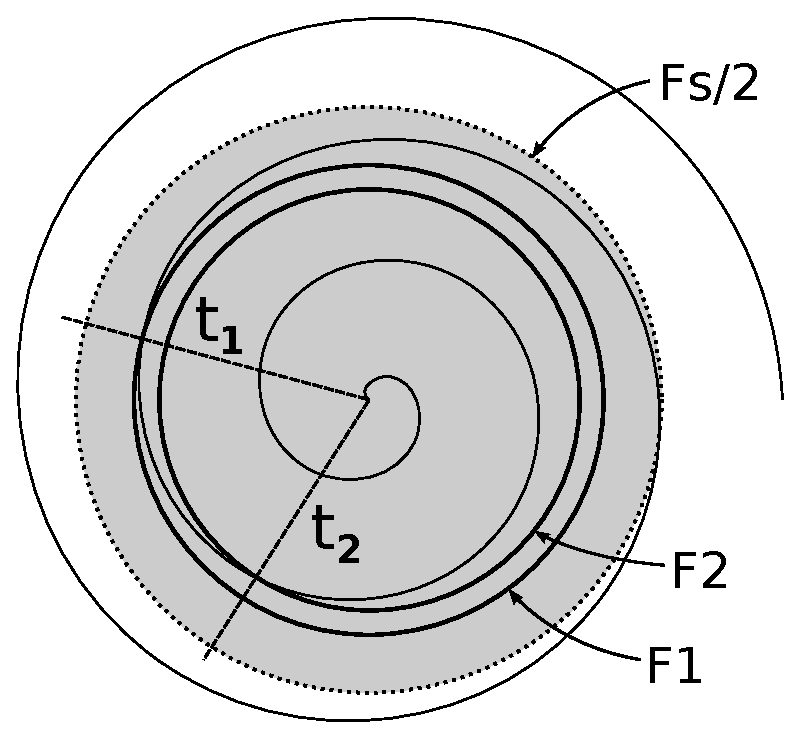
\includegraphics[width=0.7\linewidth]{../source/spiral_e}
	\caption[Emergent to Causal Time Relation]{Log polar plot of exponential chirp}
	\label{fig:spiral}
\end{figure}

Resonant signals in the emergent time domain can be re-mapped to causal time
and demodulated by correlating a time series of fast exponential chirp
transforms, allowing analysis and data mining using modern data
processing technologies such as AI-based pattern recognition.

The correlation effect can be visualized as a spinning logarithmic spiral
illuminated by a strobe light. When the strobe frequency matches the rate
constant of the spiral(s), it appears to be standing still.
Otherwise, it's a blur.

The relationship between emergent time and causal time can be thought of as a
2D plot in log-polar format.
Log-polar format renders a logarithmic spiral as a linear (Archimedean) spiral.
The spiral's radius is $\rho = k\theta$, where $k$ is a rate constant.
$\rho$ can represent either time or frequency by flipping the sign of $k$.
For purposes of signal processing, let $\rho$ represent log frequency and
$\theta$ causal time.

Log-polar mapping has proven useful in machine vision \cite{Bonmassar}
because it approximates the primate visual map \cite{Schwartz}.
Humans are visual thinkers, so their waking consciousness should map onto the
log-polar structure of emergent time signaling.

Fig.~\ref{fig:spiral} plots an exponential chirp in log-polar format.
A line can be drawn outward from the center of the spiral, crossing it at
multiple points.
The line rotates clockwise (in the case of downward chirp) at a step size
(from $t_1$ to $t_2$) corresponding to the oversampling rate.
For example, if the oversampling rate is 36 (each input value is used 36 times),
the step size is $10^{\circ}$.
Each angular sweep of the unit circle
(beginning and ending at line $t_1$ or $t_2$)
represents the input to a version of the Mellin transform called the
``Exponential Chirp Transform" (ECT) \cite{Bonmassar}, which is
basically a FFT with time-warped input.

The transform's frequency domain output is along line $t_1$ or $t_2$ from
approximately $\rho$ = 0 to Fs/2, where Fs/2 (the Nyquist frequency)
is shown by the dashed circle.
The radius of the circle represents the approximate bandwidth of the system.
Not all of the circle is used: Anti-aliasing cuts off before Fs/2, while signal
near the center is too spread out to be useful.

The ECT time-warps the chirp signal, which represents a single ``emergent tone".
In the $360^{\circ}$ sweep at line $t_1$,
the chirp is time-warped to a tone F1 in causal time.
A time $t_2-t_1$ later, at line $t_2$,
it's time-warped to a tone of frequency F2.
All time warping is exponential.
Note that ``exponential time warping" is different from dynamic time warping,
a popular means of pattern-matching mostly linear signals.

A convenient side effect of time warping is to transform interference
(periodic signals) into wideband noise.
The usual frequency peaks of EEG and HRV are thus discarded.

Emergent time, being logarithmic, has the property of frequency going as
$-\tau$ rather than $1/t$.
To change between time and frequency, just flip the sign of the exponent.
Tones are mirror images of time.
Signal processing is more convenient in terms of frequency,
so that is the focus of this paper.

%%%%%%%%%%%%%%%%%%%%%%%%%%%%%%%%%%%%%%%%%%%%%%%%%%%%%%%%%%%%%%%%%%%%%%%%%%%%%%%%
\subsection{\label{sec:level1}Mining Noise}

The basic data flow of signal conversion from one time domain to another
$(\tau \leftrightarrow t)$ is shown in Fig.~\ref{fig:sled}.
The conversion algorithm slides along the input and output data streams,
forward in time.
Data is processed in overlapping chunks.
In other words, after a block of processing,
the sliding part of Fig.~\ref{fig:sled} shifts slightly to the right.
In proportion to the amount of shift,
new input stream is exposed and new output stream is completed.
The I/O streams are low-bandwidth compared to the compute-intensive
processing block.

\begin{figure}
	\centering
	
\includegraphics[width=0.95\linewidth]{../source/sled_e}
	\caption[Emergent to Causal Time Translation Flow]{Inter-domain data flow}
	\label{fig:sled}
\end{figure}

There are two use cases: demodulation and modulation.
For demodulation $(\tau \rightarrow t)$, the input stream is in the emergent
time domain and the output stream is in the causal time domain.
The downsampler decimates the input by 1:m, where decimation factor m is
exponentially swept upward from or downward to 1.0.
The ``warp factor'' is the growth rate in m.
The input stream consists of real numbers.
The FFT performs a real-to-complex FFT to produce a warped spectrum which is
treated as time domain envelope of magnitude and phase information.
To un-warp the spectrum, the upsampler interpolates it by 1:m where decimation
factor m is exponentially swept upward to or downward from 1.0.
The output stream consists of vectors that are many accumulations of
upsampler results.

For modulation $(t \rightarrow \tau)$, the input stream is in the causal time
domain and the output stream is in the emergent time domain. The downsampler
decimates the input by 1:m, where decimation factor m is exponentially swept
upward from or downward to 1.0 and the resulting spectrum ranges from about
N/5 to N/2.
The ``warp factor'' is the growth rate in m.
The input stream consists of complex numbers.
The IFFT performs a complex-to-real IFFT to produce a warped time domain
envelope. To un-warp the it, the upsampler interpolates it by 1:m
where decimation factor m is exponentially swept upward to or downward from 1.0.
The output stream consists of many accumulations of upsampler results.

The usual use case is demodulation.
Modulation could be for testing, reconstruction or extrapolation of a signal,
or modulation of an energy source for yet unknown applications.


\section{QT Demodulation}

\begin{figure}
	\centering
	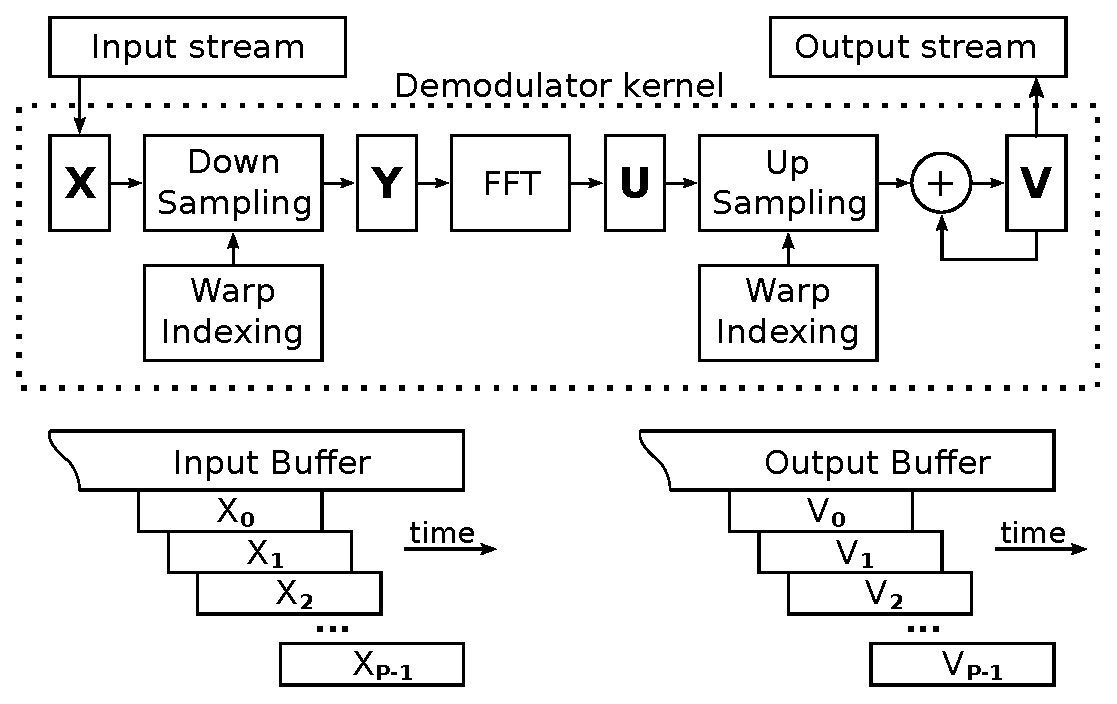
\includegraphics[width=0.95\linewidth]{../source/demod_e}
	\caption[Quantum to Relative Time Demodulation]{Demodulation data flow}
	\label{fig:demod}
\end{figure}

\begin{table}
	\label{tab:memory}
	\caption{Memory regions X, Y, U, and V in Fig.~\ref{fig:demod}
	are working buffers. For a 1k RFFT computed in place, the total is 11kB:}
	\centering
	\begin{tabular}{lccr}
		\hline\hline
		Buffer & Size & Bytes & Usage \\ [0.5ex]
		\hline
		X & 2048 x 16 & 4k & Input buffer\\
		Y/U & 1024 x 24 & 3k & FFT working buffer\\
		V & 512 x 64 & 4k & Output buffer\\
		\hline
	\end{tabular}
\end{table}

Multiple demodulator instances can be placed in an FPGA or ASIC to demodulate a
large number of $\omega$ values in parallel. This would be used in spectral
analysis, for finding signals; and deep data mining, for analyzing weak signals.
Due to the low I/O bandwidth, the algorithm lends itself to parallelism without
the complexity of high-speed signaling or memory management.
A low-cost ASIC would be feasible for consumer applications.

The mathematics of signal conversion, besides FFT, is College Algebra.
The algorithm can be coded by a typical programmer or engineer with some help
from the following derivations.

%%%%%%%%%%%%%%%%%%%%%%%%%%%%%%%%%%%%%%%%%%%%%%%%%%%%%%%%%%%%%%%%%%%%%%%%%%%%%%%%
\subsection{Downsampling}

The downsampling process of Fig.~\ref{fig:demod} translates the sample pitch of
X to the sample pitch of Y using an exponential sweep.
In the industry, this is known as exponential time-warping.

An exponential chirp sweeps from $f_0$ to $f_1$ in a time T.
M points of X get mapped onto N points of Y, where $M > N$.
Let R be a scaled version of $\omega$ for use in the exponential warp and
$\alpha$ the X input sample rate in samples per second.
Given a particular R and N, M and $\omega$ may be calculated.
Let $\epsilon = (f_1/f_0)^{1/T}$. The frequency with respect to time is:
\begin{equation}
f = f_0 \cdot e^{\epsilon t}
\end{equation}

\subsubsection{Math}

The period of the incoming chirp changes exponentially with index n of $X[n]$.
Let $y = e^{|R|/N}$ be the pitch that accumulates along X.
It has units of ``e's per sample''.
As a scale factor, let $\omega = \frac{\alpha R}{N}$,
in units of ``e's per second'' e/s.
M is the number of input samples warping onto N points.
\begin{equation}  \label{eq:M_N}
%M = \sum_{n=0}^{N-1} y^n = \frac{y\cdot(y^{N-1} - 1)}{(y - 1)} + 1
M = N \cdot\frac{-y \cdot ln\left( N(1-y) + 1 \right)}{|R|}
\end{equation}

\begin{table}
	\label{tab:MNR}
	\caption{High values of M/N are undesirable because of excess processing
	time and memory usage.
    The point of diminishing returns for M/N is between 2 and 4.
    }
	\centering
	\begin{tabular}{lcr}
		\hline\hline
		$M/N$ & $Max |R|$ & $y_{max}:y_{min}$ \\ [0.5ex]
		\hline
		2 & 1.256 & 3.51:1\\
		4 & 2.337 & 10.35:1\\
		8 & 4.229 & 68.66:1\\
		\hline
	\end{tabular}
\end{table}

An upper limit of 2 for M/N is reasonable from both a mathematical and
hardware standpoint. For example, if M is constrained to 2N, N=1024, and
$\alpha$ = 10000 samples/second, then $|\omega|$ ranges between 0 and 12.26 e/s.
When fixed-sized memories are used, smaller N allows for larger M/N, larger R,
and higher $\omega$ per input sample rate.

Re-sampling is done on N points (of Y) at a time where the respective indices of
X and Y are $\delta$ and i.
The time span is from 0 to i/N where i sweeps from 0 to N-1 and N is the number
of samples.
Let $\lambda$ be the sample pitch of X.
It will increase or decrease exponentially and should have a minimum value of
1.0, but allowed a minimum value of less than one to allow for rounding error.

This causes a chirp of matching R to be re-sampled to the upper frequency
(either $f_0$ or $f_1$ depending on the sign of R).
Given output index i, input sample index $\delta(i)$ is the accumulated sum of
$\lambda(i)$ when $\lambda$ starts at 1.0 and increases exponentially
or starts at $e^{-R}$ and decreases exponentially.
The exponential sweep can be implemented with a multiplier.
For each step:
\begin{equation}  \label{eq:lambda}
\lambda = \lambda + (\lambda\cdot\Lambda)
\end{equation}

The initial value of $\lambda$ is $e^{-R}$ when $R<0$; otherwise, it's 1.
The ``repeated multiply'' approach to exponential sweep is nearly base $e$,
but it needs a small correction factor to hit $e$.
Setting $e^R = (1 + \Lambda)^N$,
\begin{equation}  \label{eq:lambdaApprox}
\Lambda = e^{R/N} - 1
\end{equation}

As a sanity check, a downward-chirping sine wave was generated using a phase
angle proportional to $e^{n\cdot R/N} - 1$ with index $n$ starting from 0.
$\Lambda$ was set to $e^{R/N} - 1$.
A 512-point FFT (with Hann window) was performed on the de-chirped wave to
produce the expected narrow peak.

Verification of an exponential sweep built around a 27x26 multiplier used R=1.6
and N=8192. For upward sweep starting at 1.0, $\Lambda$ was $26846167/2^{37}$
according to Eq. \ref{eq:lambdaApprox}.
The accumulated $\Lambda$ was tracked and compared to the expected value from
Eq. \ref{eq:M_N}. The accumulated error after 8192 steps was less than 0.001
of an X sample pitch, so more than an order of magnitude better than necessary.
Rounding was the source of error.
Adding 1 to the LSB of $\Lambda$ lowered it to below 0.00025.
Downward sweep starting at $e^{1.6}$ had much less error.
$\Lambda$ was $-26840924/2^{37}$ and error peaked at 50 PPM.

\subsubsection{Interpolation}

The i index is stepped from 0 to N-1, where N is a power of 2 (although it
doesn't have to be) for the convenience of the FFT. $\delta(i)$ sweeps
non-linearly from 0 to M. For each X, its index $\delta$ is the running sum
of $\lambda$. For each Y point, the downsampler averages one or more X points.

There are two ways to do handle downsampling: Linear interpolation of the output
of a variable frequency low pass filter, and summation of $\lambda$
input samples.

The most common downsampling method is the low pass filter whose output is
sampled less often than its input rate.
This method attenuates alias frequencies before they make it to the output.
Anti-aliasing is good to have, but not essential in this case.
Since the alias of an exponential chirp is no longer a pure exponential
chirp (it's a linear combination of factors), it will show up in the data stream
as wideband noise rather than narrowband interference.
A low pass filter might not be needed.
The computing resourced for the filter aren't cheap.
However, a filter would improve SNR.
Such a filter must have a linear phase response.
A neat trick to use with IIR filters is forward-backward filtering,
which zeros the phase shift.
The endpoints of the filtered X are allowed some slop,
as the Hann window will lop them off anyway.

The non-filter approach is to simply sum $\lambda$ input samples of X.
Some fractional arithmetic is required to handle partial contributions.
Fig.~\ref{fig:xint} illustrates a simple interpolation that adds two fractional
endpoints to 0 or more midpoints for downsampling.
$k$ is the integer part of $\delta$.

\begin{figure}
	\centering
	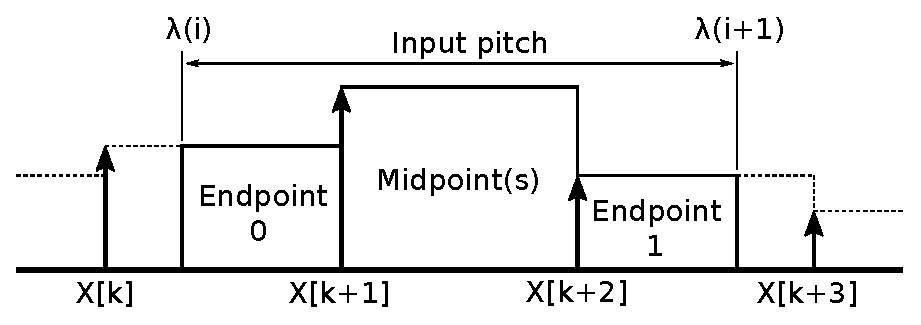
\includegraphics[width=0.95\linewidth]{../source/xint_e}
	\caption[X interpolation]{Sum of $X_\delta$ for downsampling}
	\label{fig:xint}
\end{figure}

In either case, the output of the downsampler could be scaled by
$s=\sqrt{1/\lambda}$ to flatten the noise floor.
The Central Limit Theorem reduces noise
by the square root of the number of samples in a sum.
On the other hand, one might expect energy conservation to cause the
amplitude of the incoming signal to fall off with time spreading.
So, the scaling should be optional.
Another instance of exponential sweep, with $\Lambda_s = -\Lambda/2$
and $s_0 = e^{R/2N}$,
can produce this scale factor rather easily.

\begin{figure}
	\centering
	
\includegraphics[width=0.95\linewidth]{../source/xbuf_e}
	\caption[X buffer usage]{X buffer usage}
	\label{fig:xbuf}
\end{figure}

Oversampling would normally use a sliding window on a circular buffer sized as
a power of two to allow pointer wrapping by bitwise-and.
Fig.~\ref{fig:xbuf} shows the memory layout of $X$.
After a block of processing, $\alpha\Delta$ input samples are concatenated to
$X$ and the index of $X_0$ is offset by $\alpha\Delta$,
where $\Delta$ is the time interval of the blocks.

%%%%%%%%%%%%%%%%%%%%%%%%%%%%%%%%%%%%%%%%%%%%%%%%%%%%%%%%%%%%%%%%%%%%%%%%%%%%%%%
\subsection{FFT}

After X is time warped into Y, Y is processed by a Fast Fourier Transform and
converted to data set U containing N/2 frequency bins. Y and U may share the
same physical memory if the FFT is performed in place.

Polar format is preferred for the output of the FFT,
for the benefit of the upsampler.
A Hann window $w(n)$ is applied to Y before performing the FFT.
\begin{equation}
w(n) = \frac{1}{2}\left(1 - cos\left( \frac{2\pi n}{N-1} \right)\right)
\end{equation}


The reference VHDL implementation uses a pipelined CORDIC to perform the FFT.
It also applies a Hann window to Y, converts to polar output, and is shared with
the correlator to perform polar to rectangular conversions.

A DIT FFT is the usual choice for RFFT since bit reversal is easier at the input.
With an RFFT, you get twice the outputs given real-only input.
Adjacent input samples are grouped as pairs, with even samples as real and odd
samples as imaginary components of the complex input points.
After a CFFT is performed, a separation step doubles the output size.
Our experience is that the precision of the separation step degrades with small N
(maybe we did it wrong), so a simple CFFT (with zeroed imaginary part)
may be preferable in cases of small N.

An FFT can be converted to IFFT somewhat trivially, so the same hardware can
support either modulation or demodulation.

%%%%%%%%%%%%%%%%%%%%%%%%%%%%%%%%%%%%%%%%%%%%%%%%%%%%%%%%%%%%%%%%%%%%%%%%%%%%%%%%
\subsection{Upsampling}

U is upsampled to form time-domain signal V.
Let $\epsilon$ and j be the respective indices of U and V.
For every index $\epsilon$ of U, the corresponding frequency can be normalized
to Fs/2.
Letting $\tau$ be the absolute time at $X_0$,
\begin{equation}
f = \frac{\epsilon\cdot\frac{Fs}{2}}{\frac{N}{2}}
= \frac{Fs}{2}\cdot e^{\omega(t - \tau)}
\end{equation}

It's much easier to work in terms of exponents than logs,
so the preferred re-mapping (another exponential time-warping) extracts
$U[\epsilon]$ from a linear progression of $V[j]$.
Warp indexing uses the relation:
\begin{equation}
\epsilon = \frac{N}{2}\cdot e^{\omega(t - \tau)}
\end{equation}

Time t (scaled to match the output stream's sample rate) sweeps from $\tau$
in the opposite direction of R's sign,
causing the exponent to start at 1 and decay downward.

Up-sampling $U[\epsilon]$ to $V[j]$ can't use the popular interpolation scheme
(zero stuffing) because the interpolation factor must be irrational. Instead,
partial contributions to $V[j]$ are extracted from one or two U points by
interpolation.

Let $\Delta$ be the time between conversion frames,
$\alpha$ the input sample rate,
$\beta$ the output sample rate,
$\gamma$ the input oversampling factor,
and P the number of output points in period $\Delta$.
\begin{equation}
P = \beta\Delta
\end{equation}

\begin{equation} \label{eq:eps_j}
\epsilon(j) = \left(\frac{N}{2}-1\right)\cdot e^{Rj/P}
\end{equation}

The pitch of $\epsilon$ should be 1 (when j=0) for the lowest signal loss,
but it can be lowered to reduce the computational load.
For this, $(\frac{N}{2}-1) = \frac{N}{2} e^{R/P}$. So,
\begin{equation} \label{eq:p}
\frac{R}{P} = ln\left(1 - \frac{2}{N-2}\right)
\end{equation}

For large N, $P \approx -0.5 NR$. The sample rate relations are then:
\begin{equation}
\alpha \approx \frac{2\beta\gamma}{R}
\end{equation}

\begin{equation}
\beta \approx \frac{\alpha R}{2\gamma}
\end{equation}

\begin{equation}  \label{eq:epsj}
\epsilon(j) \approx \left(\frac{N}{2}-1\right)\cdot e^{-2j/N}
\end{equation}

As a sanity check of Eq. \ref{eq:epsj}, $\epsilon(j)$ starts at (N/2-1) which
points to the highest frequency element of the FFT result.
It decays toward 0 but will never get there.
The number of elements on W memory is slightly less than N/2 to allow some I/O
headroom. Due to the limited size of W memory,
the lowest frequency is about $(1/e)$ of the highest frequency,
leaving the lower $\approx37$\% of the spectrum unused.

Let $H_X$ be the integer number of new X samples per conversion.
For example, a conversion may have M = 1000 samples.
An oversampling factor of 100 would give a $H_X$ of 10.
Let $H_V$ be the number of output samples per conversion.
Let k be a factor in Eq. \ref{eq:epsj} that's $\approx 2$.
Set the frequency shift over $H_X$ samples equal to the $\epsilon(j)$ index.
\begin{equation}
N\cdot e^{-H_X\cdot R/N} = \left(\frac{N}{2}-1\right)\cdot e^{-k \cdot H_V/N}
\end{equation}
To make $H_V$ an integer value, set k=2 and calculate rational $H_V$.
\begin{equation}
H_V = \frac{H_X \cdot R + ln\left(\frac{1}{2} + \frac{1}{N}\right)}{k}
\end{equation}

Round $H_V$ to the nearest integer and recalculate k.
\begin{equation}
k = \frac{H_X \cdot R + ln\left(\frac{1}{2} + \frac{1}{N}\right)}{H_V}
\end{equation}

The exponential decay of $\epsilon$, where $\epsilon_0 = \frac{N}{2}-1$, can be
handled by repeated multiplication.
The exponential sweep needs a small correction factor to have a base of exactly
$e$.
Setting $e^{-k} = (1 + \zeta)^N$,
\begin{equation}
\zeta = e^{k/N} - 1
\end{equation}

Since $\epsilon$ is always positive, the upchirp case of $R>0$ needs to have its
j index mirrored by using V[v-j], where v is the maximum j such as (15/32)N.

\begin{figure}
	\centering
	
\includegraphics[width=0.95\linewidth]{../source/uint_e}
	\caption[U interpolation]{Extraction of $U_\epsilon$}
	\label{fig:uint}
\end{figure}

Fig.~\ref{fig:uint} shows upsampling of U to V. It uses linear interpolation to
construct a curve to extract from.
In this case, the upsampler input pitch is less than 1.0 samples.
The height of $U_\epsilon$ is interpolated and multiplied by the pitch to get
the area under the curve, to be added to V[j].
The operation is similar to the "$\lambda < 1$" case of downsampling,
so the same hardware can support downsampling and upsampling.

%%%%%%%%%%%%%%%%%%%%%%%%%%%%%%%%%%%%%%%%%%%%%%%%%%%%%%%%%%%%%%%%%%%%%%%%%%%%%%%%
\subsection{Correlation}

Warped U is added to output buffer V by the summation,
staggered in time (by P samples) for each processing block.
When the downsampler's R value matches the chirp rate of an incoming chirp,
multiple peaks in the warped FFT output correlate in the output stream to
produce a corresponding output pulse in the V stream.
A more complex signal such as overlapping and/or modulated chirps will produce
pulse trains and/or modulation envelopes in the V stream.

\begin{figure}
	\centering
	
\includegraphics[width=0.99\linewidth]{../source/wbuf_e}
	\caption[W correlation]{Correlation of V}
	\label{fig:wbuf}
\end{figure}

Fig.~\ref{fig:wbuf} shows the output correlator, another view of buffer V.
The output stream flows from left to right,
being initialized to 0 outside the accumulation region.
After $U_\epsilon$ is added to V, the $V_0$ index moves $\beta\Delta$ points
to the left, leaving $\beta\Delta$ newly minted output points.

Elements of V may be real (magnitudes only) or complex.
Complex is used when high selectivity is required:
Multiple rotating vectors will sum to zero, while vectors pointing in the same
direction (chirps matching R) will correlate.
Correlation through vector averaging allows the use of a much smaller FFT than
scalar-only averaging.
The rate of phase rotation is proportional to the FFT result frequency,
so selectivity is higher at the upper end.
Since the low end of the FFT result isn't used,
lower selectivity there isn't a problem.

Due to the requirement that phase rotation be stationary across many FFT results
for signal detection, the exponential sweeps used in downsampling and upsampling
should use sufficient precision for correct tracking.

The correlator should be able to work with either vectors or real magnitudes
(no phase data).
This would be used in signal search, where low selectivity is desired.
The data in V, where the accumulations occur, is in rectangular format.
The data coming from the upsampler is in polar format.
The correlation process may use a CORDIC to perform polar-to-rectangular
conversion.

\section{QT Modulation}

Modulation is the reverse of demodulation.
It inputs a stream of (magnitude, angle) vectors and outputs a stream of real
samples. The downsample and upsample processes of modulation are the reverse
of demodulaton's upsample and downsample processes respectively.

\begin{figure}
	\centering
	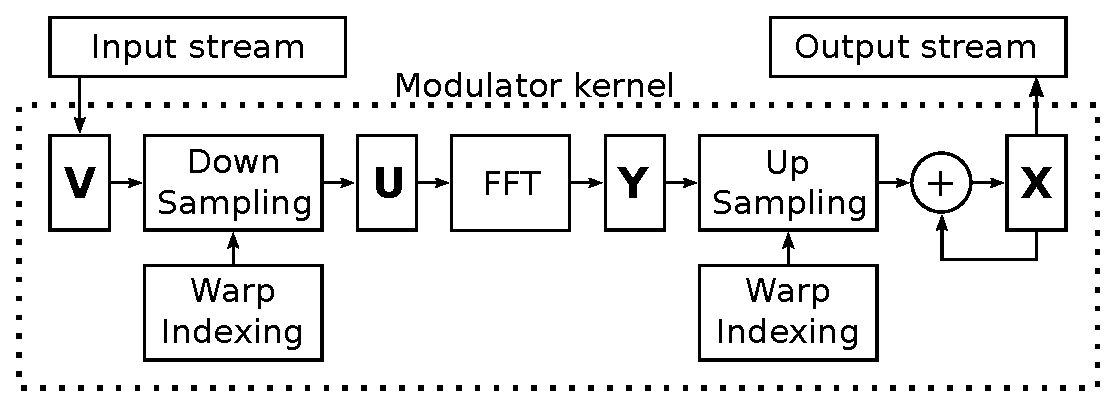
\includegraphics[width=0.95\linewidth]{../source/mod_e}
	\caption[Relative to Quantum Time Demodulation]{Modulation data flow}
	\label{fig:mod}
\end{figure}

%%%%%%%%%%%%%%%%%%%%%%%%%%%%%%%%%%%%%%%%%%%%%%%%%%%%%%%%%%%%%%%%%%%%%%%%%%%%%%%%
\subsection{Downsampling}

V is downsampled to form frequency-domain signal U.
Eq. \ref{eq:eps_j} relates integer index $j$ to fractional index $\epsilon(j)$.
Each point of V can be interpolated into a variable number of U points in a way
that accumulates V points and spits out U points as needed.

Another view is easier to describe mathematically, but needs a logarithm. Let
$\epsilon$ and j be the respective indices of U and V where $\epsilon/j < 1$.
$\epsilon$ is an integer that steps downward from $\epsilon_0$.
\begin{equation}
\epsilon_0 = \frac{N}{2} - 1
\end{equation}

Rewriting equation \ref{eq:eps_j} for $j(\epsilon)$,

\begin{equation}  \label{eq:j_eps}
j(\epsilon) = \left(\frac{N}{2}-1\right)
ln\left(\frac{\epsilon_0}{\epsilon}\right)
\end{equation}

The minimum $\epsilon$ is determined by the span of j.
Let j range from 0 to $v-1$ and $v = 0.469N$.

\begin{equation}
\epsilon(v-1) = \epsilon_0 e^\frac{-(v-1)}{0.5N - 1}
\end{equation}

\begin{equation}
\epsilon(0.469N) = \epsilon_0 e^\frac{-(0.469N-1)}{0.5N - 1}
\approx 0.391 \epsilon_0
\end{equation}

Since $\epsilon$ is always positive, the upchirp case of $R>0$ needs to have its
j index mirrored by using V[v-j], where v is the maximum j such as 0.469N.

%%%%%%%%%%%%%%%%%%%%%%%%%%%%%%%%%%%%%%%%%%%%%%%%%%%%%%%%%%%%%%%%%%%%%%%%%%%%%%%
\subsection{IFFT}

The IFFT ($U \rightarrow Y$) is an Inverse Fast Fourier Transform that
translates N/2 complex frequency values to N/2 complex points in the relative
time domain. These may be assumed to have Hermitian symmetry,
so the imaginary part of $Y$ can be ignored.
It's also possible to realize Y as N real points.

A Hann window is applied to Y after the FFT. Y is then warped and accumulated
in X in a manner similar to the demodulator's correlation function.

%%%%%%%%%%%%%%%%%%%%%%%%%%%%%%%%%%%%%%%%%%%%%%%%%%%%%%%%%%%%%%%%%%%%%%%%%%%%%%%%
\subsection{Upsampling}

The upsampling process of Fig.~\ref{fig:mod} translates the sample pitch of
Y to the sample pitch of X using the reverse of the downsampling process.

Fig.~\ref{fig:upsam} illustrates an interpolation scheme for recreating X from Y.
The slope calculation requires a $1/\lambda$ scale factor.
The expense of division can be avoided by using another instance of exponential
sweep such as that described by Eq. \ref{eq:lambdaApprox}.

The X points are the trapezoidal area under the curve in Fig.~\ref{fig:upsam}.
The \textit{Head} and \textit{Middle} regions produce output points.
The \textit{Tail} result is carried into the next \textit{Head}.

\begin{figure}
	\centering
	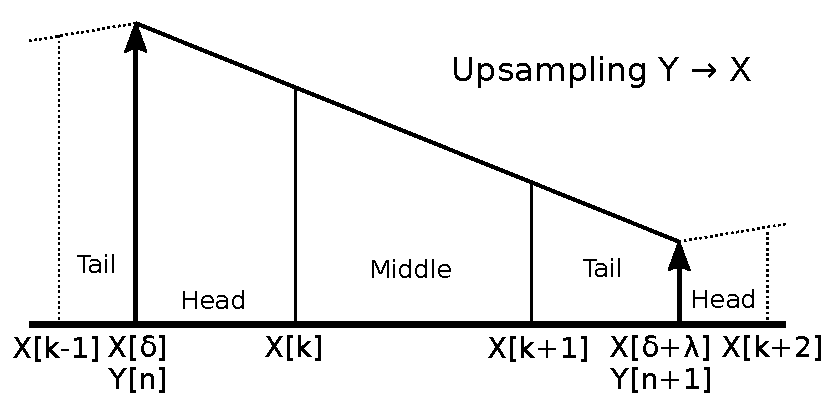
\includegraphics[width=0.8\linewidth]{../source/upsam_e}
	\caption[X interpolation]{Interpolation of Y for upsampling}
	\label{fig:upsam}
\end{figure}

Summation in X is similar to the data flow of Fig.~\ref{fig:wbuf},
but a little easier since X and Y are real (rather than complex) numbers.
X memory is wider than with demodulation to handle accumulation in memory.

\section{Implementation}

The algorithms are implemented in RTL (VHDL) for use on an FPGA or ASIC.
They may also be implemented in C, but certain functions are unwieldy on
typical computer hardware. For example, polar-to-rectangular and
rectangular-to-polar conversion is needed for upsampling complex numbers.
A simple test using GCC on a Core i7 took 1.6 $\mu$s per addition.
Table lookup (or other fast approximation) could speed that up:
Suppose 2x, so 800 ns.
In comparison, an RTL implementation using pipelined CORDIC can perform
one addition every two clocks. At 120 MHz, that's 17 ns.

A GPU could possibly process multiple data streams in parallel.
The streams themselves are serial, so there would be a memory bottleneck.
It seems FPGA is the cost/performance winner.
The RTL algorithms lend themselves to multiple on-chip instances with very
little I/O. There's also a migration path to ASIC for when consciousness
becomes ``the new media''.

The RTL uses a CORDIC-based FFT with a throughput of about 7 clocks per sample.
Since the FFT dominates the processing time, downsampling and upsampling
are performed when the FFT is idle. This allows single-port RAM access and
sharing of the CORDIC hardware.
Overall throughput for a demodulator is about 12 clocks per input sample,
so about 10 MSPS. The input sample rate (such as from an ADC) is that divided
by the oversampling factor. For example, 100x oversampling results in
an ADC sample rate of 100 kSPS.

\begin{figure}
	\centering
	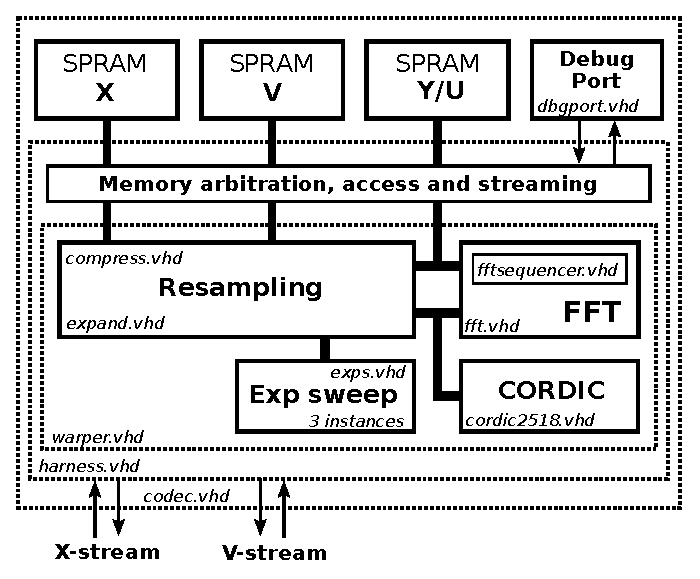
\includegraphics[width=0.8\linewidth]{../source/rtl_e}
	\caption[Emergent to Causal Time Hardware]{RTL Block Diagram}
	\label{fig:rtl}
\end{figure}

\subsection{Instrumentation}

The test port uses a half-duplex byte-oriented streaming protocol to access
hardware features for testing, verification, and debugging.
If necessary, the I/O streams may also be handled through the test port.
It uses all byte codes between 00 and FF, except for 10 to 13,
which are reserved for embedded ``escape sequences'' and flow control.
This strategy allows for XON/XOFF flow control if a UART is used as the PHY.
The PHY may be a USB FIFO chip (such as FT232H), SPI, UART, JTAG, or TWI.

The test port is used with test apps to verify separate steps of the
algorithm such as downsample, FFT, upsample, etc.
Connection to a test PC through a 2-wire UART is sufficient for FPGA testing.
The entire transform is coded in vanilla VHDL for ease of porting.

The demodulator/modulator shown in Fig.~\ref{fig:rtl} uses three memory
spaces to allow easier I/O access by the I/O streams and account for the
difference in word widths between X and V data.
The \verb|warper| uses wide data busses on the X and V memories to facilitate
correlation of outgoing data using long accumulators in either X or V memory.
Incoming data is packed two points per memory word.

\subsection {FPGA utilization}

A complete CODEC was implemented in vanilla VHDL with a single clock domain.
Free versions of synthesis tools were used to synthesize the design for use in
some sample FPGAs.
The clock rate is limited by the exponential sweep module,
which uses a single-cycle feedback loop whose path includes a 26x27 multiplier,
4:1 mux, adder, and 3:1 mux. Those two muxes will do better on FPGAs with
6-input LUTs. Synthesis for parts with LUT6 had a 50\% reduction in LUT usage
compared to LUT4-only.

\begin{table}[t]\centering
	\label{tab:FPGAfit}
	\caption{FPGA rough synthesis results. One-off distributor pricing gives a
	rough cost per MHz, using Digikey pricing, across the number of CODEC
	instances that will fit in the FPGA.}
	\centering
	\begin{tabular}{lccrrr}
		\hline\hline
		Device & Logic & DSPs & Clock & Cores & \$/MHz\\ [0.5ex]
		\hline
        Artix 7   & 8K LUT6 & 40   & 150 MHz & 12 & 0.11\\
		Cyclone 10& 14K LE & 69 9x9 & 49 MHz &  4 & 0.25\\
		LFE5      & 12K LE & 40     & 39 MHz &  1 & 0.30\\
        PolarFire & 14K LUT4 & 37   & 51 MHz &  7 & 0.40\\
		Cyclone 5 & 5K ALM & 18     & 72 MHz &  2 & 0.55\\
		MAX10     & 13K LE & 69 9x9 & 51 MHz &  1 & 1.20\\
		\hline
	\end{tabular}
\end{table}



\bibliographystyle{abbrv}
\bibliography{../source/etime}

\end{document}
